\documentclass[10pt,DIV10,a4paper]{scrartcl}
\usepackage[utf8]{inputenc}
\usepackage[german]{babel}
\usepackage{amsmath}
\usepackage{amsfonts}
\usepackage{amssymb}
\usepackage{microtype}
\usepackage{graphics}

\title{PMS -- Exercise Sheet 10}
\date{}

\begin{document}

\maketitle

\section*{Exercise 1}

$$I = \sum_{i} m_{i}
\begin{pmatrix}
    y_i^2+z_i^2 & -x_i y_i    & -x_i z_i \\
   -y_i x_i     & x_i^2+z_i^2 & -y_i z_i \\
   -z_i x_i     & - z_i y_i     &  x_i^2+y_i^2 \\
\end{pmatrix} = \left(\begin{array}{rrr}
59.2& 0 & 0 \\
0 & 3.52 & 0 \\
0 & 0 & 62.72
\end{array}\right)$$

\section*{Exercise 2}

$$\vec{L} = I\vec{\omega} = \left(\begin{array}{rrr}
59.2& 0 & 0 \\
0 & 3.52 & 0 \\
0 & 0 & 62.72
\end{array}\right)
\left(\begin{array}{r}
0\\
1\\
0
\end{array}\right) = \left(\begin{array}{r}
0\\
3.52\\
0
\end{array}\right)
$$

\section*{Exercise 3}

$$I' = \left(\begin{array}{rrr}
61.888 & -1.152 & 0 \\
-1.152 & 0.576 & 0 \\
0 & 0 & 62.464
\end{array}\right)$$

\section*{Exercise 4}

$$\vec{\omega}' = I'^{-1}\vec{L} \approx \left(\begin{array}{r}
0.12\\
6.35\\
0
\end{array}\right)$$

$$|\vec{\omega}'| \approx 6.35\ \text{s}^{-1}$$

\section*{Exercise 5}

As our dancer has moved her left arm upward and her right arm downward, the mass points of her right arm are further away from her center of mass. Thus the rotational axis shifts towards this direction.
\begin{align*}
M\cdot r_{com}&=\sum_i m_i \left( \begin{array}{r}
x_i\\
y_i\\
z_i\\
\end{array} \right) \\
\Rightarrow r_{com}&=\left(\begin{array}{r}
0\\
\frac{52}{60}\\
0
\end{array} \right)
\end{align*}
(Over the next few rotations, due to the tilted axis of rotation, gravity would pull the dancer towards earth and tilt the axis even further.)
In this case I would rather suggest rotational inbalance:

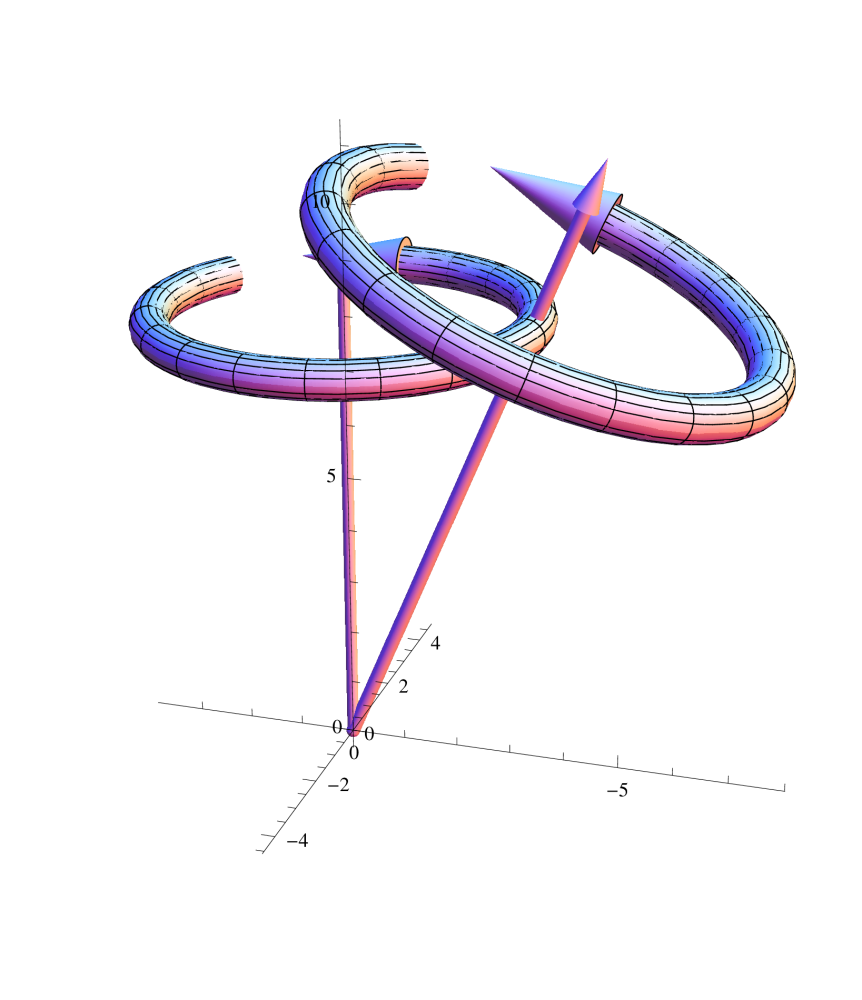
\includegraphics{unwucht.eps}

Error source: The inertia tensor describes rotation around an objects center of gravity, while in our case the dancer's rotational axis will always run through the contact point between feet and floor. Additionally, due to friction with air and floor, the dancer would probably not spin that fast.
\begin{itemize}
\item Not many masspoints; bad approximation of real world scenario
\end{itemize}

\end{document}
